\documentclass[11pt,a4paper]{extarticle}

\usepackage[top=1.5in]{geometry}
\usepackage{amsmath}
\usepackage{graphicx}
\usepackage{titling}
\usepackage{changepage}
\usepackage{multicol}
\usepackage{listings}
\graphicspath{{images/}}

\setlength{\droptitle}{-10em}

\title{\textbf{Graph Theory \& Algorithms}}
\date{23 December 2017}
\author{Aniket Pandey}

\begin{document}
\maketitle

%\section{Acknowledgement}
%\textit{I would like to thank Sunil Pandey () for %mentoring me in the project and in helping me prepare this %report. I would also like to thank ACA for giving me the %opportunity to learn the topic in detail.}

\section{Introduction}
Graph Theory is the study of Graphs, the mathematical objects modelling the pairwise relation of Vertices(also called nodes) and Edges where two nodes are connected by edges. A graph can be directed or undirected, cyclic or acyclic, linear or weighted etc. 

Graph Theoretical concepts are widely used to study and model various applications, in different areas. For example, in Computer Science, problems like travelling salesman problem, the shortest spanning tree in a weighted graph and in Mathematics like hamiltonian graphs and Fermat's Little Theorem \& Nielson-Schreier Theorem. 

\section{Notations}
\subsection{Big-O Notation}
Big-O Notations are used in mathematics to characterize functions according to their growth rate. In Graph Theory, efficiency of an algorithm is measured in terms of the input length $n$ as $n\rightarrow \infty $.\par Formal definition would be\\If $f:N\rightarrow N$ and $g:N\rightarrow N$ are two functions, then $f=$O$(g)$ if and only if $f(n)<c \cdot g(n)$ for a constant $c$ as $n\rightarrow\infty$.
\subsection{Other Notations}
There are a few more notations which complement Big-O Notation. I will give a brief information about these.\par
For functions $f$ \& $g$ from $N$ to $N$

\begin{align}
f =&\:\Omega(g)\quad  \textrm{if} \,\,  g=O(f)\\
f =&\:\Theta(g)\quad \textrm{if} \,\,  f=O(g) \,\, \& \,\, g=O(f)\\
f =&\:o(g)\:\,\quad \textrm{if there exists }\varepsilon \textrm{ such that} \,\, f(n)<\varepsilon\cdot g(n) \\
f =&\:\omega(g)\quad \:\textrm{if} \,\,  g=o(f)
\end{align}

\section{Terminologies}
Here are a few basic terminologies that are used to represent navigation through the Graph. \\
\begin{adjustwidth}{1.5em}{0pt}
\begin{description}
\item [Walk] A walk is any route through a graph from vertex to vertex along edges. A walk can end on the same vertex on which it began or on a different vertex. A walk can travel over any edge and any vertex any number of times.
\item [Path] A path is a walk that does not include any vertex twice, except that its first vertex might be the same as its last.
\item [Trail] A trail is a walk that does not pass over the same edge twice. A trail might visit the same vertex twice, but only if it comes and goes from a different edge each time.
\item [Cycle] A cycle is a path that begins and ends on the same vertex.	
\end{description}
\end{adjustwidth}

\section{Data Structures used in Graphs}
\subsection{Adjacency List}
An Adjacency List is a collection of unordered lists used to represent a finite graph. Each list describes the set of neighbors of a vertex in the graph.
\begin{center}
	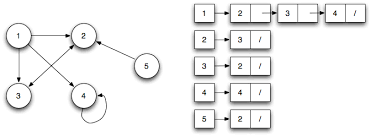
\includegraphics[width=8cm, height=3cm]{list}
\end{center} 

\subsection{Adjacency Matrix}
An Adjacency Matrix is a square matrix used to represent a finite graph. The elements of the matrix indicate whether pairs of vertices are adjacent or not in the graph.
\begin{center}
	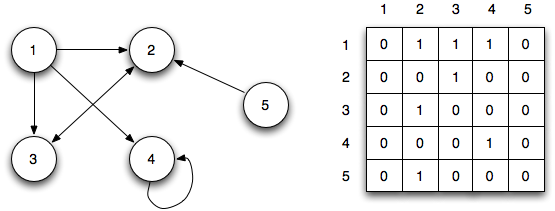
\includegraphics[width=8cm, height=3cm]{matrix}
\end{center}
 
\subsection{Stacks and Queues} 
Stacks and Queues are dynamic sets in which the element removed from the set by the \textit{delete} operation is prespecified. In a Stack, the element deleted from the set is the one inserted most recently, while in a Queue, the element that is to be deleted is the element which has been in the Queue for the longest time. \\

A \textbf{Stack} is a container of objects that are inserted and removed according to the last-in first-out (LIFO) principle. In the pushdown stacks only two operations are allowed: push the item into the stack, and pop the item out of the stack.

A \textbf{Queue} is a container of objects that are inserted and removed according to the first-in first-out (FIFO) principle. In the queue only two operations are allowed, enqueue and dequeue. Enqueue means to insert an item into the back of the queue, dequeue means removing the front item.
\newpage
\begin{multicols}{2}

\begin{center}
	\textbf{STACK}
\end{center}

\lstinputlisting[language=Python, showstringspaces=false]{code/stack.py}

\columnbreak

\begin{center}
	\textbf{QUEUE}
\end{center}

\lstinputlisting[language=Python, showstringspaces=false]{code/queue.py}

\end{multicols}

\section{BFS and DFS}


\end{document}
